\documentclass[border=15pt, multi, tikz]{standalone}
\usepackage{import}
\subimport{../../layers/}{init}
\usetikzlibrary{positioning}
\usetikzlibrary{3d} %for including external image 

\def\ConvColor{rgb:brown,5;yellow,2.5;black,5}
\def\ConvReluColor{rgb:orange,5;red,5;white,5}
\def\BatchNormColor{rgb:red,1;white,5.3}
\def\TanhColor{rgb:magenta,5;white,7}

\begin{document}
\begin{tikzpicture}


\tikzstyle{connection}=[ultra thick,every node/.style={sloped,allow upside down},draw=\edgecolor,opacity=0.5]


%% Draw Layer Blocks
%%%%%%%%%%%%%%%%%%%%%%%%%%%%%%%%%%%%%%%%%%%%%%%%%%%%%%%%%%%%%%%%%%%%%%%%%%%%%%%%%%%%%%%%



% conv1, LeakyRelu
\pic[shift={(0,0,0)}] at (0,0,0) {Box={name=conv_block1,caption=NoiseVector,%
        xlabel={{"100","dummy"}}, ylabel=1,zlabel=1,fill=\ConvColor,%
        height=5,width={10},depth=5}};
        

% conv2, BatchNorm, LeakyRelu
\pic[shift={(1.5,0,0)}] at (conv_block1-east) {RightBandedBox={name=conv_block2,caption=deConv + Batch Norm + ReLU,%
        xlabel={{"2048","dummy"}}, ylabel=4, fill=\ConvColor,bandfill=\BatchNormColor,%
        height=10,width={30},depth=10}};
        
\pic[shift={(0,0,0)}] at (conv_block2-east) {Box={name=relu1,%
        fill=\ConvReluColor,opacity=0.8,height=10,width=1,depth=10}};


% conv3_1,conv3_2,pool3
\pic[shift={(1.7,0,0)}] at (relu1-east) {RightBandedBox={name=conv_block3,caption=dConv + BN + ReLU,%
        xlabel={{"1024","dummy"}}, ylabel=8, fill=\ConvColor,bandfill=\BatchNormColor,%
        height=20,width={25},depth=20}};
        
\pic[shift={(0,0,0)}] at (conv_block3-east) {Box={name=relu2,%
        fill=\ConvReluColor,opacity=0.8,height=20,width=1,depth=20}};
        
% conv4_1,conv4_2,conv4_3,pool4
\pic[shift={(2.3,0,0)}] at (relu2-east) {RightBandedBox={name=conv_block4,caption=dConv + BN + ReLU,%
        xlabel={{"512","dummy"}}, ylabel=16, fill=\ConvColor,bandfill=\BatchNormColor,%
        height=25,width={20},depth=25}};
        
\pic[shift={(0,0,0)}] at (conv_block4-east) {Box={name=relu3,%
        fill=\ConvReluColor,opacity=0.8,height=25,width=1,depth=25}};
        
% conv5_1,conv5_2,conv5_3,pool5
\pic[shift={(2.7,0,0)}] at (relu3-east) {RightBandedBox={name=conv_block5,caption={dConv + BN + ReLU},%
        xlabel={{"256", "dummy"}}, ylabel=32,fill=\ConvColor,bandfill=\BatchNormColor,%
        height=30,width={15},depth=30}};
        
\pic[shift={(0,0,0)}] at (conv_block5-east) {Box={name=relu4,%
        fill=\ConvReluColor,opacity=0.8,height=30,width=1,depth=30}};

% conv5_1,conv5_2,conv5_3,pool5
\pic[shift={(3.25,0,0)}] at (relu4-east) {RightBandedBox={name=conv_block6,caption={dConv + BN + ReLU},%
        xlabel={{"128", "dummy"}}, ylabel=64, fill=\ConvColor, bandfill=\BatchNormColor,%
        height=40,width={10},depth=40}};
        
\pic[shift={(0,0,0)}] at (conv_block6-east) {Box={name=relu5,%
        fill=\ConvReluColor,opacity=0.8,height=40,width=1,depth=40}};
        
\pic[shift={(2,0,0)}] at (relu5-east) {Box={name=conv_block7,  caption= dConv,%
        fill=\ConvColor,xlabel=3, ylabel=128, opacity=0.4,height=50,width=1,depth=50}};
        
\pic[shift={(1.5,0,0)}] at (conv_block7-east) {Box={name=tanh, caption= Tanh,%
        fill=\TanhColor,opacity=0.8,height=50,width=1,depth=50}};
        
\node[canvas is zy plane at x=43] (temp) at (-4,0,0) {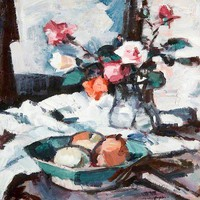
\includegraphics[width=10cm,height=10cm]{art.jpg}};

%%%%%%%%%%%%%%%%%%%%%%%%%%%%%%%%%%%%%%%%%%%%%%%%%%%%%%%%%%%%%%%%%%%%%%%%%%%%%%%%%%%%%%%%
%% Draw connections
%%%%%%%%%%%%%%%%%%%%%%%%%%%%%%%%%%%%%%%%%%%%%%%%%%%%%%%%%%%%%%%%%%%%%%%%%%%%%%%%%%%%%%%%
\draw [connection]  (conv_block1-east)    -- node {\midarrow} (conv_block2-west);
\draw [connection]  (relu1-east)    -- node {\midarrow} (conv_block3-west);
\draw [connection]  (relu2-east)    -- node {\midarrow} (conv_block4-west);
\draw [connection]  (relu3-east)    -- node {\midarrow} (conv_block5-west);
\draw [connection]  (relu4-east)    -- node {\midarrow} (conv_block6-west);


%%%%%%%%%%%%%%%%%%%%%%%%%%%%%%%%%%%%%%%%%%%%%%%%%%%%%%%%%%%%%%%%%%%%%%%%%%%%%%%%%%%%%%%%

\end{tikzpicture}
\end{document}\grid